\section{ASTRI-Horn data reduction and analysis} 
\label{sect:astridata}

A side emitting Fiber Optics system(FOC) is located  along the PMMA 
circumference. It is illuminated by a Light Emitting Diode (LED) 
system and used for the on-field relative calibration of the gain. 
Its light uniformly illuminates the PDMs units at a controlled intensity.


\subsection{Open sky data} (Alessio)
\label{subs:skydata}

%715+705 +788 499 + 972 + 1180+1157   
%940 +944 +984 + 995+ 514

%1001+ 981 +792+ 808+ 755+ 818 +592 +408+ 88
%1730 + 1762+ 1804 +1814 1420
%1329 +1496 +684 

\begin{table}[ht]
\label{tab:astrilog}
\caption{ASTRI-Horn observation log}
\centering
\begin{tabular}{lcccc}
\hline\hline
Observation ID & Starting Date & Exposure      & Number of events & pointing \\
               & (year/month/day h:m:s) & (s)  \\
\hline     
%https://www.overleaf.com/project/5e3005eb54e0d8000155a7ff
1453 & 2018/12/07 20:06:11  &   6016     & 348442 & Crab Off    \\
1454 & 2018/12/07 22:09:16  &   4377     & 226651 &  Crab \\ %226650  \\
1455 & 2018/12/07 23:30:08  &   6243     & 412451 &  Crab \\ %412446    \\
1456 & 2018/12/08 01:24:48  &  8530     & 237318 & Crab Off \\ %  237186 \\
1457 & 2018/12/07 03:50:20  &  3509     & 126295 & Fixed ALtAzi\\ % 126264   \\
1464 & 2018/12/08 20:30:37 &  2255 & 97257 & Crab Off \\ %97251 \\  
1465 & 2018/12/08 21:17:34 &  9624 & 430245 & Crab\\ % 430222\\  
1466 & 2018/12/09 00:07:25 &  3161 & 251442 & Crab \\ %251418  
1467 & 2018/12/08 01:09:44 &  8959 & 243713 & Crab Off \\ %243399
1468 & 2018/12/08 03:40:11 &  1237 & 33168 &  Fixed AltAzi\\ %33126
1658 & 2019/03/05 18:13:58 &  112 & 1435 & Merak \\  
1659 & 2019/03/05 18:19:26 &  154 & 3149 & Zeta Tauri \\  
1660 & 2019/03/05 18:24:37 &  6224  & 419636 & Crab \\ %419631  
1661 & 2019/03/05 20:10:15 &  168 & 14389 & Zeta Tauri \\  
1662 & 2019/03/05 20:19:59 &  4008 & 198186 & Crab Off \\   
1663 & 2019/03/05 21:29:34 &  2337 & 165264 &  Fixed AltAzi \\  
1670 & 2019/03/06 18:08:27 &  628    &   8191      &  Merak\\
1671 & 2019/03/05 18:21:51 &  126        &   2412   & Zeta Tauri \\
1672 & 2019/03/05 18:25:56 &  5935    &   296073   &  Crab \\ %296046
1673 & 2019/03/05 20:06:58 &  183      &   3272     & Zeta Tauri\\ %3270
1674 & 2019/03/05 20:13:37 &  13812      &    152393 & Crab Off  \\ %152110     \\
%1466 & 2018/12/09 20:47:50 &  1218 & 50000 \\  

\hline\hline
\end{tabular}
\end{table}

\subsection{Closed camera data} (Domenico)\\
The first step of the analysis chain is the camera calibration. 
It concerns the relative calibration 
of the pixels in the camera, i.e. the signal extraction and conversion into 
physical units, and the estimation of the level of statistical 
fluctuations of the pixel signals.
For the ASTRI-Horn, the signal waveforms are acquired with a 
sampling in peak detector mode, in order to obtain a pulse height distributions (PHD) for 
each physical pixel.
However the calibrated data must be expressed in term of 
photo-electrons(p.e.). Therefore the conversion factors from the maximum 
amplitude of the pulse to p.e. and from the integral of the pulse to p.e. 
must be known. 
The method to extract the conversion factor, also called gain, is to calculate the equivalent 
signal (maximum amplitude in ADC) for a single photon.
To do so, the ASTRI-Horn plans to have two types of low light level runs:\\
\textbf{\textit{FOC runs}} are acquired during the physics data taking.
In order to avoid that these events overlap with physics event, the light is flashed 
at a lower rate than the expected physics trigger rate. The light 
produced by the FOC must be uniform and should have an average of 
few p.e. per pixel. This allows to monitor continuously the gain of the 
electronics chain. Figure~\ref{fig1} shows the pulse height spectrum acquired in one of the FOC run listed in Table~\ref{table2} with a fixed voltage $V_{0}$= 57 V 
and a temperature of 15$^\circ$C for a camera pixel in the High Gain electronics chain. 
The distribution shown is the reconstructed maximum amplitude for all the 
recorded waveforms of a physical pixel. While the first peak is the pedestal, the following 
ones are the single and multiple p.e. contributions. The distance between 
the peaks allow to extract the conversion factor.\\
\begin{figure*}[ht!!]
\centering
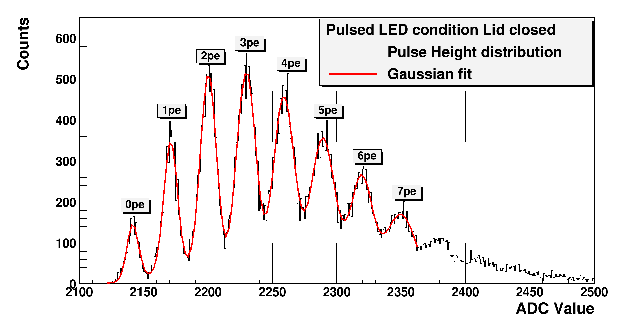
\includegraphics[angle=0, width=12.5cm]{PIXEL60_PDM20_HG_DICEMBRE_2018.eps}
\vspace{0.5cm}
\caption{ Pulse height spectrum at a fixed temperature of 15$^\circ$C
and $V_{0}$=57 V for a camera pixel, during a FOC run in the HG electronics chain. 
The black curve represents the distribution of the peak detector output and the red curve shows the corresponding
multiple peaks Gaussian fit.}
\label{fig1}
\end{figure*}

\textbf{\textit{Dark counts runs}} are acquired
when the lids of the camera are closed.
The light-tight lid, in addition to protecting the FSC, it ensures that no light
can enter it when the lid is latched shut. In this way, it is possible to read out
the pulse height of all the signals pixel for each triggered dark event.
In absence of light, using the Low Gain electronics chain, the majority of events are 
contained in one peak position, named pedestal. 
It, that does not vary with temperature(\cite{Impiombato2016}), is considered as offset electronics chain in the analysis of cherenkov images for the astronomical
observations.
Each pulse height spectrum of the camera pixels, is fitted with a Gaussian function, allowing to obtain the exact peak position value in the ADC counts with the relative width (see Fig.~\ref{fig2}).





\begin{figure*}[h!!]
\centering
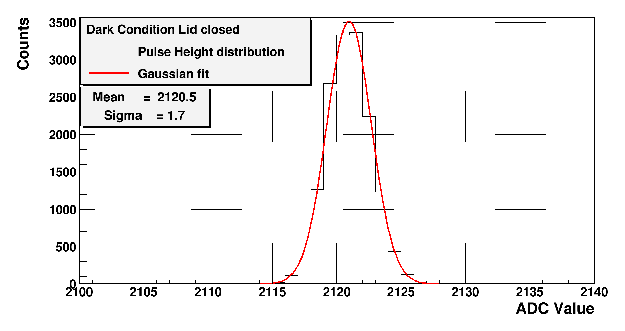
\includegraphics[angle=0, width=12cm]{PIXEL60_PDM20_LG_DICEMBRE_2018.eps}
\vspace{0.5cm}
\caption{ Single photo-electron peak spectrum for a camera pixel taken in peak detector mode in one of the Dark run listed in 
Table~\ref{table2}. The black curve represents the distribution of the peak detector
output and the red curve shows the corresponding Gaussian fit.}
\label{fig2}
\end{figure*}
\label{subs:skydata}





\begin{table*}[htbp!!]
\centering
\caption{ASTRI-Horn FOC/Dark runs}
\label{table2}
\begin{tabular}{lccc}
\hline\hline
Run ID & Starting Date & Run type      & Number of events \\
               & (year/month/day h:m:s)   \\
\hline     
1380 & 2018/12/01 20:59:18  &   Dark    & 15305      \\
1394 & 2018/12/02 20:01:09  &   FOC     & 60065     \\
1616 & 2019/02/28 12:37:02  &   Dark    & 50000     \\
1763 & 2019/03/23 20:01:21  &   FOC     & 120123    \\
  

\hline\hline
\end{tabular}
\end{table*}
